% !TEX root = Thesis.tex

%==============================================================================
\chapter{Erbium \acl*{bec}}
\label{chap:erbium_bec}
%==============================================================================

This chapter has the objective of briefly review some relevant properties of Erbium, which will clarify what makes it relevant in the study of ultra cold atoms. After this, the basic theory of Bose-Einstein condensation will be discussed, along with a brief description of the experimental phases and tools required to create and observe an Erbium \ac{bec}. This experimental realization will be the foundation on which the following chapters will be grounded when discussing further experimental achievements.

%==============================================================================
\section{Properties of atomic erbium} \label{sec:erbium_properties}
%==============================================================================
Erbium is a chemical element with an atomic number of 68, which belongs to the series of the Lanthanides. It is also part of the group called Rare-earth elements and it was first discovered by G. Monsander in 1843 \cite{mosander1843xxx}. The name of ``Erbium'' comes from the name of the Swedish village of Ytterby, the place where it was extracted. At that time, the similarity of rare-earth metals' chemical properties made their distinction extremely difficult. For this reason, what G. Monsander thought to be pure Erbium oxide was in fact a mixture of different rare-earth metal oxides. The element is not obtained in a reasonably pure form until 1937 by W. Klemm and H. Bommer \cite{klemm1937bommer}.

Considering some basic properties of this element, under standard conditions erbium is in a solid state. It has a silver shining surface, which oxidizes with air contact. This rare-earth metal has a melting point of 1802 K and boiling point of 3136 K. As a result, to be able to work with a free atomic gas of erbium requires to heap up the solid erbium metal to high temperatures \cite{emsley1998}.

The number of stables isotopes of Erbium is 6 and they can be seen in Table \ref{tab:Isotopes_Erbium}. All of them are bosons with nuclear spin of zero, in exception of $^{\text{167}}\text{Er}$, which is a fermion with spin of 7/2. The chosen isotope for this experiment is $^{\text{168}}\text{Er}$ because of its bosonic nature, high abundance and favorable scattering properties.

\begin{table}[htbp] \centering
	\begin{tabular}{@{}c|c|c|c@{}}\hline
		Isotope                  & Abundance [\%]          & Atomic Mass [u] & Nuclear Spin [$\hbar$] \\ \hline\hline
		$\text{Er}^{\text{162}}$ &  0.14                   & 161.928775      & 0   \\
		$\text{Er}^{\text{164}}$ &  1.61                   & 163.929198      & 0   \\ 
		$\text{Er}^{\text{166}}$ & 33.60                   & 165.930290      & 0   \\
		$\text{Er}^{\text{167}}$ & 22.95                   & 166.932046      & 7/2   \\
		$\text{Er}^{\text{168}}$ & 26.80                   & 167.932368      & 0   \\  
		$\text{Er}^{\text{170}}$ & 14.90                   & 169.935461      & 0   \\  \hline
	\end{tabular}
	\caption[Table with the stable isotopes of Erbium]{Table with the stable isotopes of Erbium that can be found on Nature with their respective Abundance ratio, Atomic mass and Nuclear Spin. Spectroscopy data taken from \cite{sansonetti2005handbook}.}\label{tab:Isotopes_Erbium}
\end{table}

In addition to these properties, erbium atoms have a rather complex energetic level scheme due to its open 4f shell. This one lacks 2 electrons to be completely filled, which makes erbium to have an electronic ground state with an orbital angular momentum value of $L = 5$ and a high magnetic moment of seven Bohr magneton $7\mu_B$ \cite{ban2005laser}. This high value for the orbital angular momentum in the ground state of erbium provides several advantages for Raman-coupling processes. Leading to longer coherence times and stronger synthetic magnetic fields when comparing with other alkali metals like rubidium or cesium, commonly used in ultracold atoms experiments  \cite{cui2013synthetic}.


A scheme of erbium energy levels together with the atomic transitions used in this experiment can be seen in figure \ref{fig:erbium_scheme}. The scheme shows that the electronic ground state of erbium is $\text{[Xe] }\text{4f}^{12} \text{6s}^2$, where [Xe]
represents the complete electronic configuration of Xenon\footnote{$\text{[Xe] = }\text{1s}^2 \text{ 2s}^2 \text{ 2p}^6 \text{ 3s}^2 \text{ 3p}^6 \text{ 3d}^{10} \text{ 4s}^2 \text{ 4p}^6 \text{ 4d}^{10} \text{ 5s}^2 \text{ 5p}^6$}. Moreover, the used optical transitions are represented by colored arrows in the figure and its spectroscopic data is shown in table \ref{tab:Transitions}. From now on, these three transitions will respectively be referred to as the 401nm, 583nm, and 841nm transitions.

Finally, it must be noted that aside from the discussed application in ultracold atoms, erbium is used in multiple commercial applications. One prominent example is the use or erbium as a fiber amplifier in doped silicon fibers \cite{mears1987low}. Furthermore, in nuclear physics it is used as neutron absorbing control rods \cite{emsley2011nature}.

%\sisetup{per-mode = symbol}%

\begin{table}[htbp] \centering
	\begin{tabular}{@{}l|c|c|S|S|S@{}}\hline
		\multicolumn{3}{c|}{Parameters} & \multicolumn{3}{c}{Transitions} \\ \hline
		Name & Symbol & Unit & \multicolumn{1}{c|}{401nm} & \multicolumn{1}{c|}{583nm} & \multicolumn{1}{c}{841nm} \\ \hline\hline
		Wavelength in vacuum & $\lambda$	& \si{\nano\meter}					& 400.91		& 582.84		& 841.22\\
		Lifetime 			& $\tau$	& \si{\micro\second}				& 0.045			& 0.857			& 20   \\ 
		Natural linewidth 	& $\Delta \nu_0$	& \si{\kilo\hertz}					& \num{33370} 	& 185.71 		& 7.96   \\
		Decay rate 			& $\gamma$	& \si{\per\second}					& \num{2.22e8} 	& \num{1.17e6}  & \num{5.00e4} \\
		Saturation intensity & $I_{S}$	& \si{\milli\watt\per\centi\meter}	& 71.80			& 0.12			& 1.74  \\  
		Doppler temperature	& $T_D$	& \si{\micro\kelvin} 				& 848.69  		& 4.46  		& 0.19    \\  
		Doppler velocity	& $v_D$	& \si{\centi\meter\per\second}		& 21.5 			& 1.49 			& 0.31 \\  \hline
	\end{tabular}
	\caption[Spectroscopic data for the optical transitions of Erbium]{Spectroscopic data for the optical transitions of Erbium used in this experiment. These transitions are called the 401nm, 583nm, and 841nm transitions and can be seen in figure \ref{fig:erbium_scheme}. Data taken from \cite{mcclelland2006natural, lawler2010atomic, den2010radiative, ban2005laser, lipert1993isotope}}\label{tab:Transitions}
\end{table}


\begin{figure}[h!]\centering
	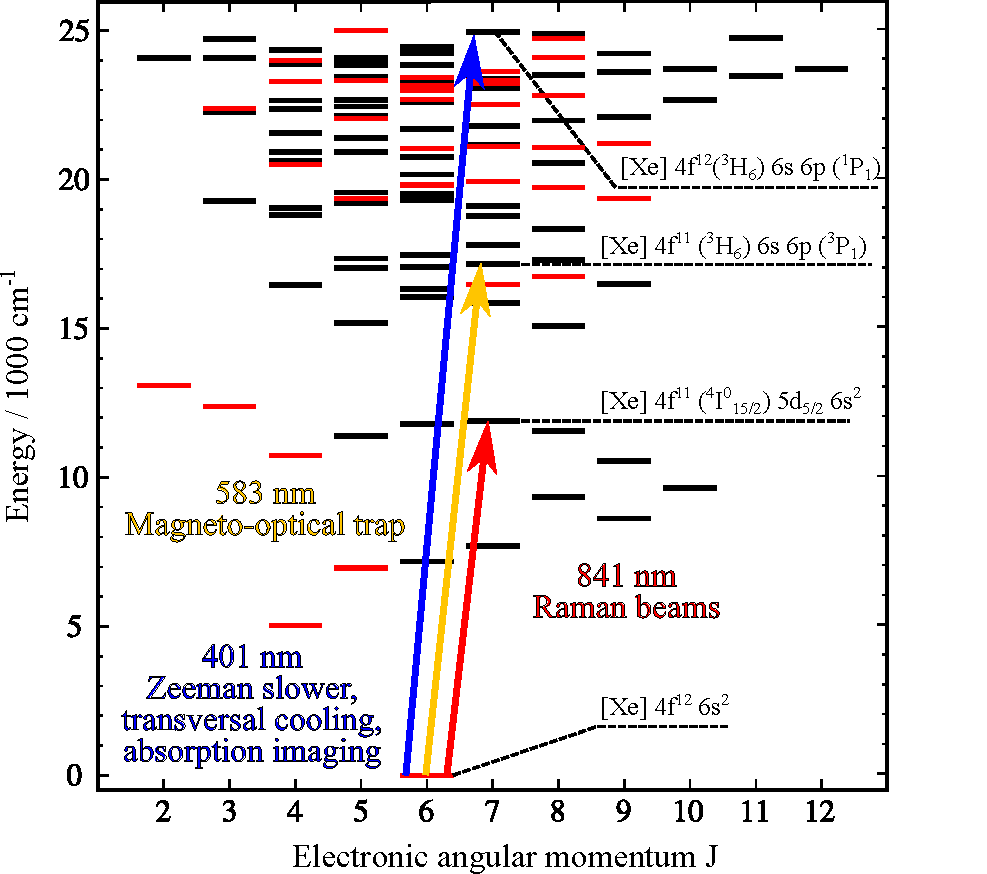
\includegraphics[width=1.\columnwidth]{erbium_term_scheme.pdf}
	\caption[Erbium energy scheme]{Energy level scheme of Erbium represented as a function of the total angular momentum J. This scheme shows only a range of energies relevant for the experiment of up to 25000 $\text{cm}^{\text{-1}}$. The different arrows show us the used transitions and for which phase of the experiment they are used for. The red lines represent energy states with even parity and the black lines those with odd parity. Data taken from \cite{NIST}. }\label{fig:erbium_scheme}
\end{figure}


%==============================================================================
\section{Bose-Einstein Condensation} \label{sec:bose-einstein_condensation}
%==============================================================================

A \acl*{bec} is generally defined as a state of matter formed when a gas of bosons with a low density is cooled to near-zero temperatures (typically a few hundreds nanokelvins). To understand this definition and the next theoretical principles is necessary to define what is a boson. 

In quantum mechanics, bosons are particles with an integer value in their spin. Because of this,  also have a symmetric wave function under the interchange of two particles, which allows bosons to have the same quantum state. Unlike its counterpart fermions, which have a half odd integer spin and an anti-symmetric wave function. Leading to Pauli's exclusion principle that avoids more than one fermion to occupy the same quantum state \cite{Pauli1925}.

It was the Indian physicist S. N. Bose the first one who described in a successful way an ideal gas of non interacting free photons in 1924.


\hfill

\clearpage

%==============================================================================
\section{Experimental preparation} \label{sec:experimental_preparation}
%==============================================================================

\begin{figure}[h!]\centering
	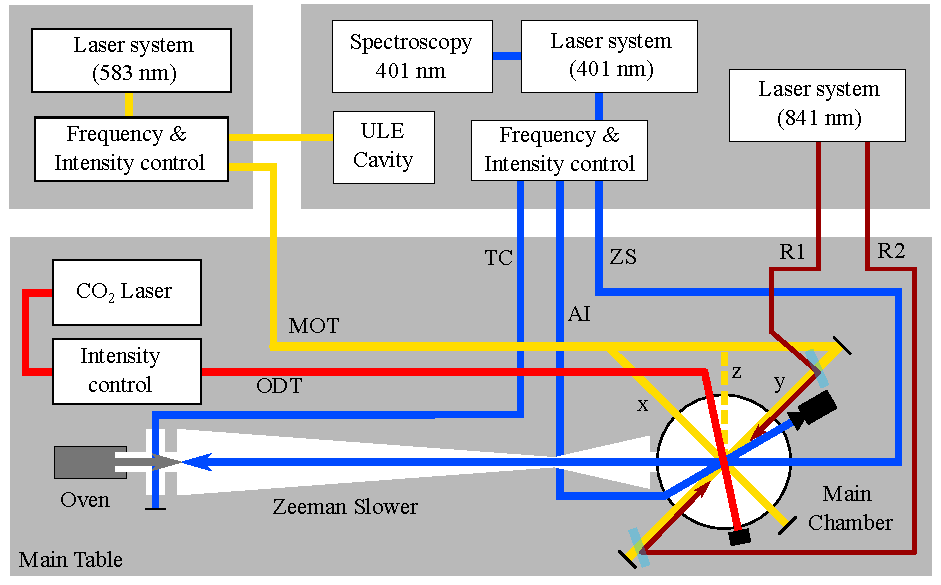
\includegraphics[width=1.\columnwidth]{table_set_up.pdf}
	\caption[Scheme of the experimental set up]{Scheme of the experimental set up}\label{fig:table_set_up}
\end{figure}

%%% Local Variables: 
%%% mode: latex
%%% TeX-master: "Thesis"
%%% End: 